% ===========================================================================
% GridSpike -- anonymized manuscript for Engineering Applications of
% Artificial Intelligence (Elsevier), double-anonymized review.
%
% Author names, affiliations, CRediT, funding and competing-interest details
% are in the SEPARATE title page file: titlepage.tex (compile it on its own).
% This file must contain nothing that identifies the authors.
%
% Build:  make            (latexmk -pdf main.tex)
% ===========================================================================
\documentclass[final,3p,times,twocolumn]{elsarticle}

\usepackage[T1]{fontenc}
\usepackage[utf8]{inputenc}
\usepackage{amsmath,amssymb}
\usepackage{graphicx}
\usepackage[dvipsnames]{xcolor}
\usepackage{booktabs}
\usepackage{array}
\usepackage{multirow}
\usepackage{tabularx}
\usepackage{rotating}
\usepackage{algorithm}
\usepackage{algpseudocode}
\usepackage{tikz}
\usetikzlibrary{positioning,arrows.meta,fit,backgrounds,calc}
\usepackage[switch]{lineno}
\usepackage[hidelinks]{hyperref}
% Cross-references into the supplementary document (compiled separately):
% \ref{...} on a label that lives only in supplementary.tex resolves to its
% S-number there. xr would also import the other file's \bibcite entries
% (renumbering shared citations), so the build filters supplementary.aux
% down to its \newlabel lines into supplabels.aux and xr reads that file:
%   Select-String '\\newlabel' supplementary.aux > supplabels.aux
\usepackage{xr}
\externaldocument{supplabels}

\linenumbers

% Float packing: this manuscript is table-dense (twenty full-width floats), and
% LaTeX's defaults strand text pages behind them. These are typographic limits,
% not content changes.
\renewcommand{\topfraction}{0.92}
\renewcommand{\bottomfraction}{0.75}
\renewcommand{\textfraction}{0.06}
\renewcommand{\floatpagefraction}{0.72}
\renewcommand{\dbltopfraction}{0.92}
\renewcommand{\dblfloatpagefraction}{0.68}
\setcounter{topnumber}{3}
\setcounter{dbltopnumber}{3}
\setcounter{totalnumber}{4}
\setlength{\textfloatsep}{9pt plus 2pt minus 3pt}
\setlength{\dbltextfloatsep}{9pt plus 2pt minus 3pt}
\setlength{\floatsep}{7pt plus 2pt minus 2pt}
\setlength{\dblfloatsep}{7pt plus 2pt minus 2pt}
\setlength{\intextsep}{7pt plus 2pt minus 2pt}
\setlength{\abovecaptionskip}{5pt}
\setlength{\belowcaptionskip}{0pt}
% Review mode's line stretch (\baselinestretch = 1.5) applies inside floats as
% well; with this many dense tables it pushes them over the page height.
% Float contents therefore stay single-spaced while the body text keeps the
% required stretch (captions included, which is also the common review style).
\AtBeginEnvironment{table}{\linespread{1}}
\AtBeginEnvironment{table*}{\linespread{1}}
\AtBeginEnvironment{figure}{\linespread{1}}
\AtBeginEnvironment{figure*}{\linespread{1}}
\AtBeginEnvironment{algorithm}{\linespread{1}}
% natbib inter-entry spacing: 76 references, so this is worth a third of a page.
\AtBeginDocument{\setlength{\bibsep}{0pt plus 0.3ex}}

% ---------------------------------------------------------------------------
% macros.tex -- shared macros for the manuscript.
%
% The cardinal rule of this project: NO FABRICATED NUMBERS. Every numeric result
% must come from a generated file. Until the experiment battery lands, every
% place where a number belongs carries \TODOnum{...}, which typesets a loud red
% marker that cannot be mistaken for a value in a compiled PDF.
% ---------------------------------------------------------------------------

% \TODOnum{label} -- a results-shaped hole. The argument is a short tag naming
% what belongs there, so the battery-to-manuscript wiring is unambiguous.
% \TODOnum{} (empty argument) is the bare marker.
\newcommand{\TODOnum}[1]{%
  \textcolor[rgb]{0.85,0.0,0.0}{\textbf{[\,??\,\ifx\relax#1\relax\else\,\textsf{\footnotesize #1}\,\fi]}}%
}

% \TODOfig{filename}{what the figure will show} -- a placeholder frame for a
% figure that only the battery can produce. Never an \includegraphics of a
% missing file, so the document always compiles and the hole is loud.
\newcommand{\TODOfig}[2]{%
  \begingroup
  \setlength{\fboxrule}{1.2pt}%
  \setlength{\fboxsep}{10pt}%
  \textcolor[rgb]{0.85,0.0,0.0}{%
    \fbox{\parbox[c][7.5\baselineskip][c]{0.86\linewidth}{\centering
      \textbf{FIGURE PENDING}\\[4pt]
      \texttt{figures/#1}\\[6pt]
      \normalfont\itshape #2}}}%
  \endgroup
}

% Short-hand for the system name, so a rename is a one-line edit.
\newcommand{\sysname}{GridSpike}

% Units / symbols used repeatedly.
\newcommand{\uJ}{\ensuremath{\mu\mathrm{J}}}
\newcommand{\pJ}{\ensuremath{\mathrm{pJ}}}
\newcommand{\ms}{\ensuremath{\mathrm{ms}}}
\newcommand{\macroF}{macro-F\textsubscript{1}}
\newcommand{\SynOps}{SynOps}

% Event-class names, typeset consistently.
\newcommand{\cls}[1]{\textsc{\small #1}}

% Table template shared by every table (generated and hand-written):
% tabularx at \linewidth, \scriptsize, \arraystretch 1.15, booktabs rules,
% caption above, notes in \tablenota below the rule.
\newcolumntype{L}{>{\raggedright\arraybackslash}X}
\newcolumntype{C}{>{\centering\arraybackslash}X}
% Y{r}: ragged X column at r times the average X width (ratios sum to the X count).
\newcolumntype{Y}[1]{>{\raggedright\arraybackslash\hsize=#1\hsize}X}
\newcommand{\tablenota}[1]{\par\smallskip\begin{minipage}{\linewidth}\scriptsize #1\end{minipage}}


\journal{Engineering Applications of Artificial Intelligence}

\begin{document}

\begin{frontmatter}

\title{\sysname: Defense-aware stress-testing of federated edge
intelligence for event classification in IEC 61850 substations}

% --- Double-anonymized submission: no author block here by design. ---------

\begin{abstract}
Distribution utilities need event classification on substation telemetry --
for disturbance triage, targeted inspection and reliability analytics --
but no utility holds enough labelled events to train one alone,
and pooling measurements collides with confidentiality and
critical-infrastructure rules. Federated learning is the institutional
answer, provided the federation survives heterogeneous data, a bounded edge
and adversarial participants. We present \sysname, a federated framework and
open benchmark -- five feeders in quasi-static OpenDSS, non-IID by
feeder identity and Dirichlet label skew -- stress-tested. Three
classifiers -- convolutional--recurrent, spiking, selective state-space --
learned over ten substations behind a Byzantine-admission pipeline:
fidelity scoring, simulated PBFT agreement, robust aggregation,
hash-chained per round. Across an expanded battery of $6{,}836$ run
records the models trace an accuracy--energy--latency trade-off. On the
leakage-controlled chronological split -- our headline protocol -- the
reference and the state-space model tie
(\macroF{} $0.596$ vs.\ $0.590$, paired $p=0.56$), and the spiking model --
at $0.7\%$ of the reference's energy -- collapses to $0.13$; the higher
$0.77/0.60/0.16$ of the random split is a leakage-inflated ceiling. Only
the reference's GPU \mbox{p99} ($3.3$\,ms) fits a $4$\,ms
fast-message envelope ($82\%$); the others exceed it. Under a defense-aware
adversary the pipeline beats neither plain averaging nor robust aggregation
alone -- it buys auditability, not accuracy -- and usable local differential
privacy is incompatible with the gate. In-cone magnitude at $10\times$
breaks plain averaging, not the geometric median: honest rejection falls
$0.80 \rightarrow 0.48$, attacker admission does not. The classifier provides
event awareness and takes no part in trip decisions. Batteries
regenerate from committed manifests; the original battery's configuration
hashes verify at $67\%$.
\end{abstract}

\begin{keyword}
Federated learning \sep State-space models \sep Spiking neural networks \sep
Byzantine robustness \sep IEC 61850 \sep Power distribution \sep
Differential privacy
\end{keyword}

\end{frontmatter}

% ---------------------------------------------------------------------------
% Highlights -- EAAI submission checklist: 3 to 5 bullets, each at most 85
% characters INCLUDING SPACES. Verified by `make check-highlights`.
% Deliberately number-free: no headline value may be asserted before the
% experiment battery has produced it.
% ---------------------------------------------------------------------------
\section*{Highlights}
\begin{itemize}\setlength{\itemsep}{2pt}
\item Two dense model families tie on accuracy inside a three-way edge trade-off
\item A quasi-static OpenDSS generator makes the federation non-IID by construction
\item A high-magnitude in-cone attacker breaks plain averaging, not the geometric median
\item Under a defense-aware attacker, agreement buys auditability, not model accuracy
\item Usable local differential privacy is incompatible with the Byzantine admission gate
\end{itemize}


\section{Introduction}
\label{sec:intro}

\begin{figure*}[!t]
\centering
% Generated by scripts/figura1_drawio.py (numbers: scripts/numeros_fig1.csv;
% thumbnails: scripts/figura1_insumos.py); editable source figures/fig1_overview.drawio.
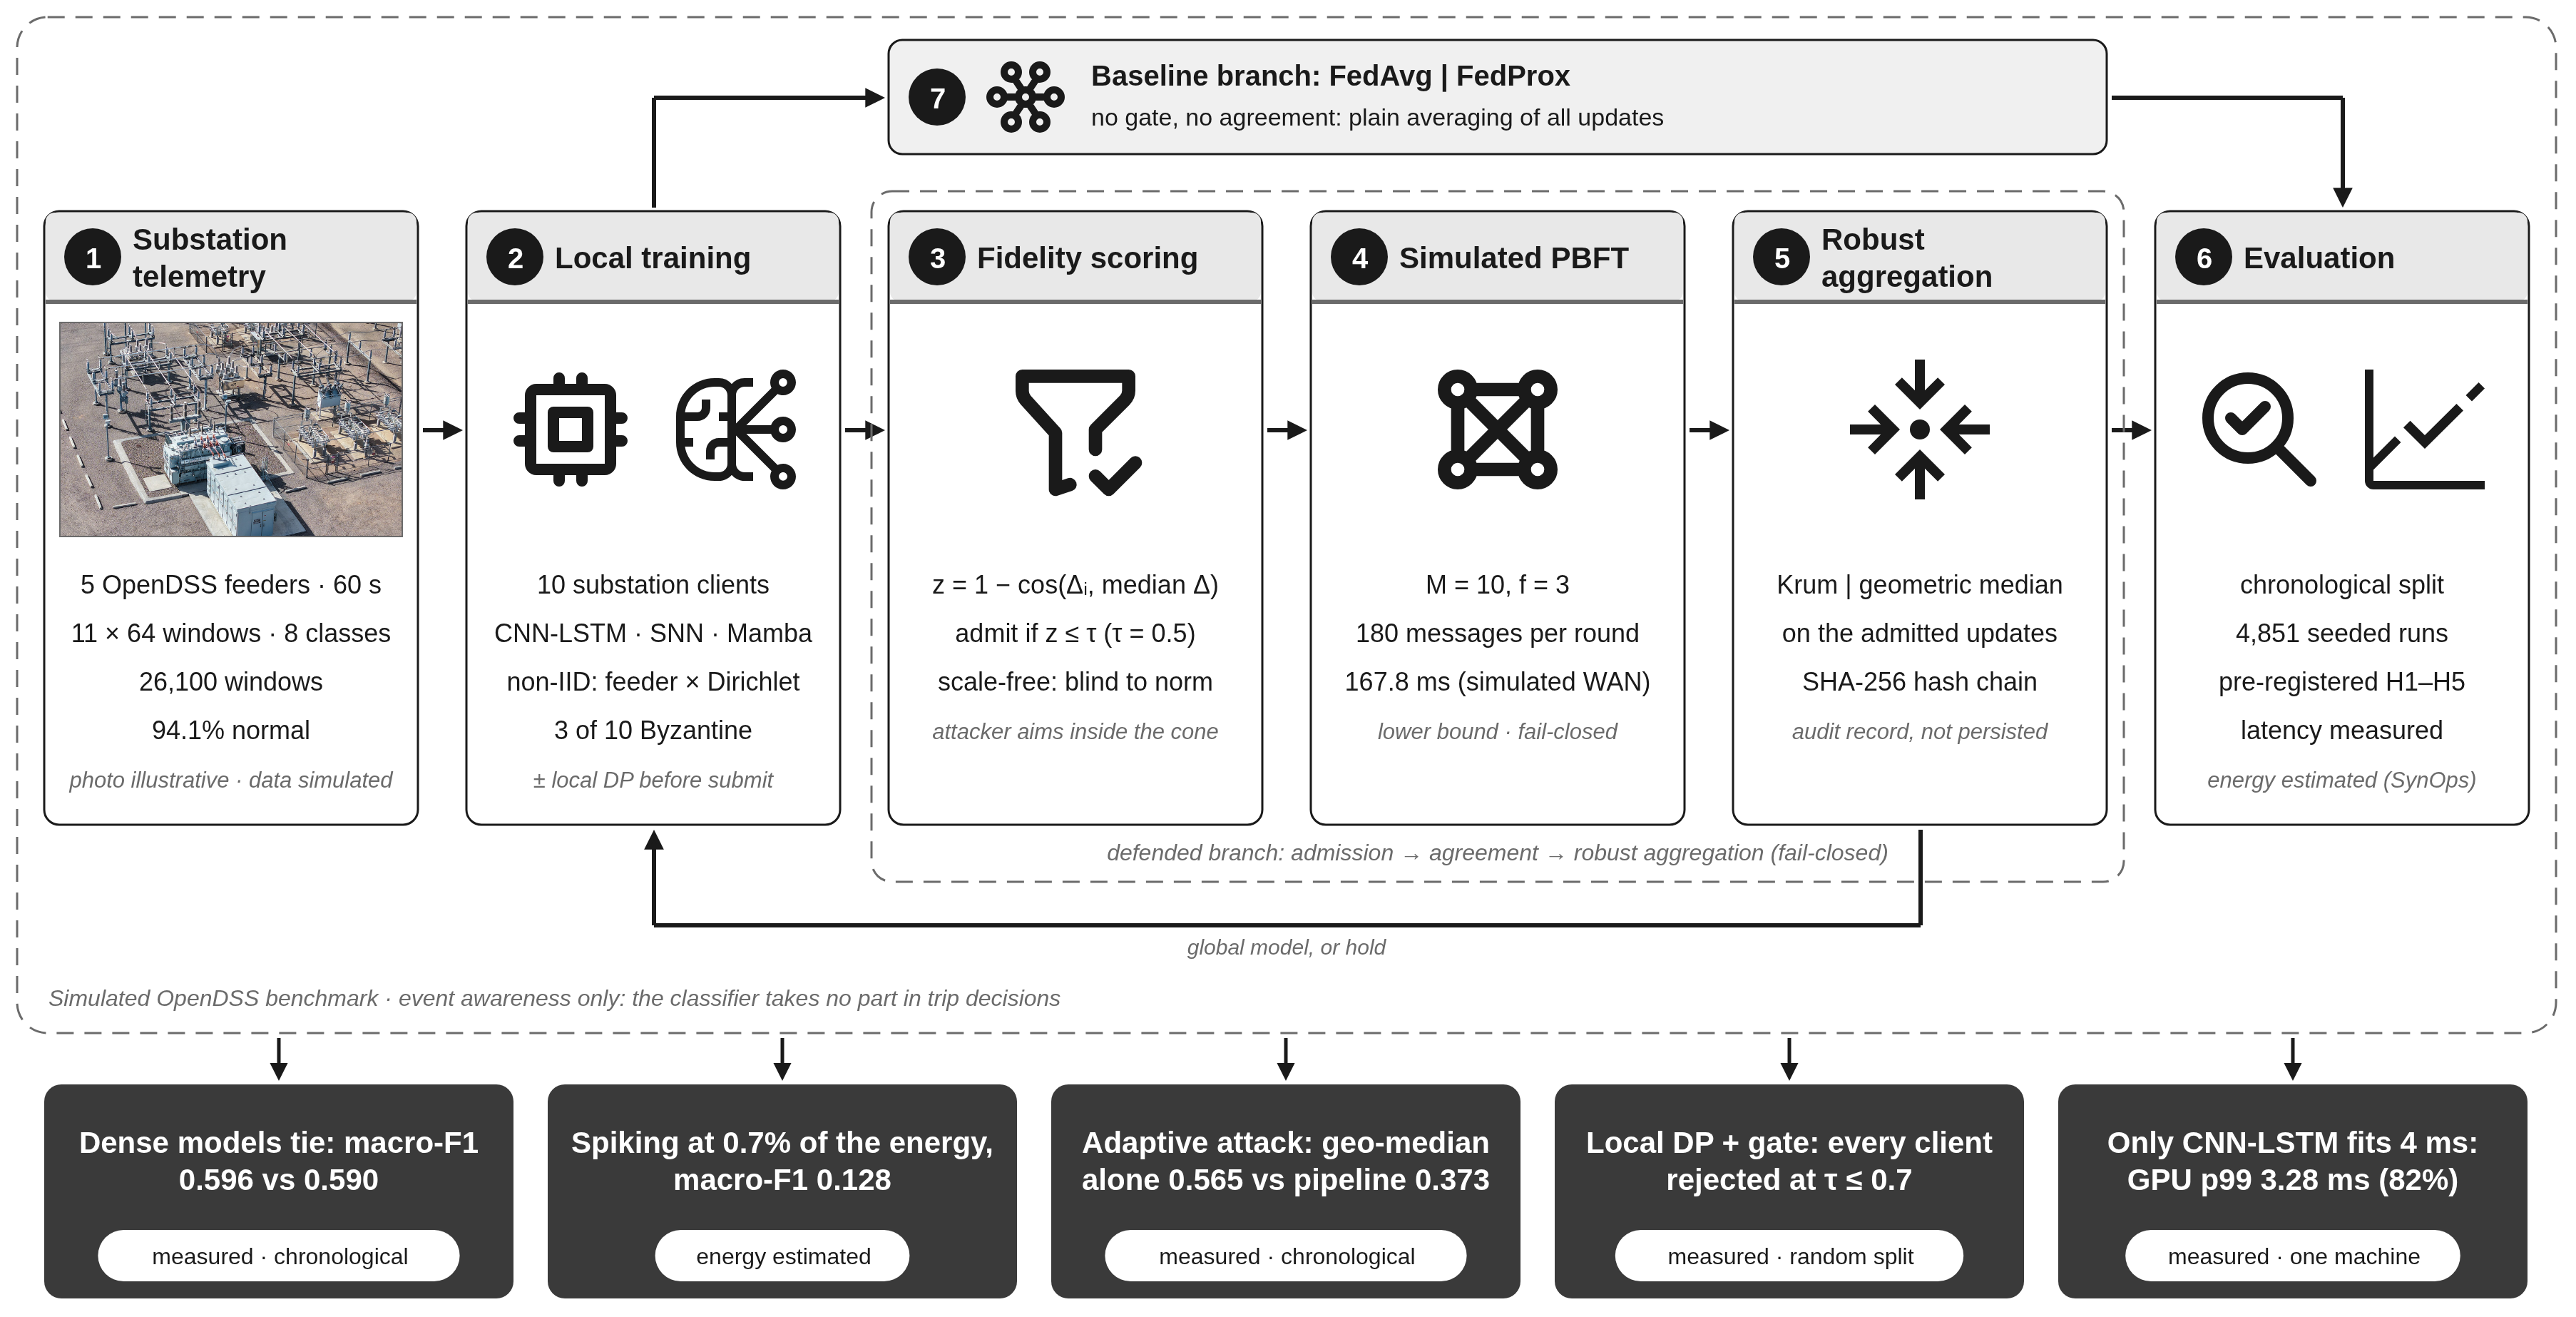
\includegraphics[width=\textwidth]{figures/fig1_overview.png}
\caption{\sysname{} overview: substation telemetry (1) through local
training (2), fidelity scoring (3), simulated PBFT (4) and robust
aggregation (5) to evaluation (6), against the FedAvg/FedProx baseline (7);
bottom, headline results with evidence tags. Photo illustrative (CC0).}
\label{fig:pipeline}
\end{figure*}

Substation gateways conforming to the IEC 61850 family publish
time-aligned electrical measurements -- per-phase voltages and currents,
power, zero-sequence quantities, frequency -- that carry the signature of
the events an operator cares about: ground faults, phase-to-phase faults,
cold-load pickup, sustained sags and swells. Classifying those events
\emph{at the substation edge} shortens the path from measurement to
situational awareness: it feeds control-room triage, inspection
scheduling and reliability analytics. It is an \emph{event-awareness}
function, not a protection function -- the classifier labels windows in a
telemetry stream and takes no part in any trip decision. At the 60\,s
cadence this telemetry delivers, one $T{=}64$ window spans about an hour
of acquisition, which fixes the timescale everything here operates on.

Four constraints make the target hard, and they are usually studied one
at a time. \emph{Data cannot be pooled}: no single distribution utility
holds enough labelled events to train a deep classifier, and pooling
across utilities collides with confidentiality and
critical-infrastructure rules -- the natural fit is cross-silo federated
learning \cite{mcmahan2017}, a few institutional participants with
substantial local data and no willingness to release it. \emph{The
federation is non-identically distributed by construction}: substations
sit on different feeders with different load mixes, generation
penetration and event populations, so heterogeneity is the physical
situation, not a nuisance parameter. \emph{The edge is energy- and
latency-bounded}: devices are fanless and retrofit-powered, the stream is
overwhelmingly normal operation -- the regime an event-driven spiking
classifier should exploit \cite{eshraghian2023,horowitz2014} -- and a
classifier co-resident with protection-adjacent signalling must fit
inside the 4\,ms fast-message transfer-time yardstick the
intrusion-detection literature already uses
\cite{ustun2021,moore2026}. \emph{The federation is adversarially
exposed}: a compromised gateway is a Byzantine participant, a
sophisticated one knows the defense it faces \cite{fang2020,shejwalkar2021},
there is no trusted server-held clean dataset \cite{cao2021fltrust}, and
the local-differential-privacy mechanism that makes participation
acceptable makes honest clients look like attackers
\cite{guerraoui2021podc}.

This paper presents \sysname, a framework that handles all four
constraints in one system, together with the physics-based benchmark
generator that produces its data (Figure~\ref{fig:pipeline} draws the
end-to-end path). \sysname{} is a research artifact: the
simulation, federated engine, attack suite, validation pipeline,
experiment runner and analysis code are released together, and the
batteries behind Section~\ref{sec:results} regenerate from committed
manifests, with per-run configuration hashes verifying canonically for
$67\%$ of the original battery's records.

\subsection{Contributions}
\label{sec:contributions}

\begin{enumerate}\setlength{\itemsep}{1pt}
\item \textbf{A reproducible, physics-grounded federated benchmark
  generator} (Section~\ref{sec:testbed}). Five standard feeders solved
  in quasi-static time series with sample-accurate event injection, a
  modelled measurement chain and a realistic rare-event prior; the
  federation is non-IID on two axes -- feeder identity and Dirichlet
  label skew \cite{hsu2019}. We claim the generator, not the task
  \cite{husnoo2023fedisa,husnoo2023feddisc,li2025fdia}.
\item \textbf{A three-architecture edge comparison under robust
  federation} (Sections~\ref{sec:arch}, \ref{sec:results}). A
  convolutional--recurrent reference, a surrogate-gradient spiking
  network and a selective state-space (Mamba) model on the same
  benchmark and admission pipeline -- a federated spiking classifier on
  substation measurements, and a state-space model in this setting, have
  no precedent \cite{venkatesha2021,nguyen2025robust,mahapatra2021}. The
  honest finding is a trade-off on the leakage-controlled split: the two
  dense models tie, the spiking model is two orders of magnitude cheaper
  in energy but collapses, and only the reference fits a co-resident
  4\,ms envelope.
\item \textbf{A defense-aware attacker carried end-to-end}
  (Section~\ref{sec:threat}). An adversary that knows the admission rule
  constructs in closed form an update inside the admissible cone, plus a
  separate magnitude lever exploiting the scale-freeness of cosine
  scoring \cite{fang2020,shejwalkar2021,baruch2019,xie2019}, evaluated
  against both robust aggregators with the evasion-versus-damage
  asymmetry measured.
\item \textbf{Consensus overhead measured next to the accuracy it buys}
  (Sections~\ref{sec:arch}, \ref{sec:results}). Exact message counts and
  simulated wide-area latency per round, plus the ablation the
  agreement-plus-aggregation literature \cite{kfc2025,li2024brfl}
  usually omits: the pipeline against the robust aggregator standing
  alone. Agreement buys auditability, not accuracy.
\item \textbf{An empirical privacy-versus-admission account}
  (Section~\ref{sec:results}). That differential privacy composes poorly
  with Byzantine resilience is a theorem, and not ours
  \cite{guerraoui2021podc}; we provide the
  measured account of honest false-rejection against attacker admission
  across noise multiplier and threshold, annotated with the R\'enyi
  privacy budget \cite{mironov2017}. At every usable privacy level the
  gate fails closed: the mechanisms are incompatible, not tunable.
\item \textbf{A compute-share budget for waveform-window classifiers}
  (Section~\ref{sec:results}). Measured latency percentiles for all
  three models against the 4\,ms fast-message envelope -- the adjacent
  literature benchmarks packet-level detectors against that figure
  \cite{ustun2021,moore2026}; waveform classifiers have not been placed
  in it before.
\end{enumerate}

\subsection{What this paper does not claim}
\label{sec:nonclaims}

Stating the boundary is cheaper than being corrected at it. We do not
claim first federated learning for power-system fault classification
\cite{husnoo2023fedisa,husnoo2023feddisc}, the discovery of the
privacy--robustness tension \cite{guerraoui2021podc}, or novelty in
combining Byzantine agreement with robust aggregation
\cite{kfc2025,li2024brfl}. We do not claim a hardware energy measurement
(figures are SynOps estimates \cite{horowitz2014}, arithmetic only),
field validation (data come from a simulator;
Section~\ref{sec:limitations}), or end-to-end verification of the
hash-chained ledger (recomputed by property tests, never persisted). We
do not claim Byzantine-fault-tolerant security under equivocation or
partition (the agreement stage is simulated), a protection function (the
4\,ms figure is a compute-share reference, not a deadline), or that the
spiking classifier beats the reference -- the design target is accuracy
\emph{parity} at lower estimated energy, tested as an equivalence claim.

\subsection{Related work}
\label{sec:related}

Five active lines meet here; each is developed fully, with its most
dangerous neighbour named, in Supplementary Section~\ref{sec:sup-related}
and Table~\ref{tab:positioning}. \emph{Federated grid analytics} is
established \cite{husnoo2023fedisa,husnoo2023feddisc,li2025fdia} -- but
every member consumes a fixed dataset; none constructs the federation
from physics. \emph{Spiking classifiers for power systems} exist on
phasor measurements \cite{mahapatra2021} -- centralized, the strongest
precedent for our energy claim -- and federated spiking learning exists
on vision benchmarks \cite{venkatesha2021,aouedi2023hfedsnn}, recently
under Byzantine attack \cite{nguyen2025robust} but with a non-omniscient
adversary and no consensus layer. \emph{Byzantine-robust
aggregation} is settled \cite{blanchard2017,pillutla2022}; trust
bootstrapping \cite{cao2021fltrust} is excluded (no clean server-side
data exists); defense-aware poisoning defines our adversary
\cite{fang2020,shejwalkar2021,baruch2019,xie2019}.
\emph{Agreement-plus-aggregation} combinations are crowded
\cite{kfc2025,li2024brfl} but report neither the protocol's overhead nor
a defense-aware attacker. \emph{DP--Byzantine composition} is
theoretically understood \cite{guerraoui2021podc} and actively
engineered \cite{gu2024dpbrem}, but no member
of that line supplies a measured operating curve in an application
system. \emph{Latency against the 4\,ms envelope} is standard only for
packet-level intrusion detection \cite{ustun2021,moore2026}. The claim
is not any column of that space but the intersection: no prior system
occupies it.

Formal definitions, the extended related work, the realism parameter
audit, battery and provenance detail, and the complete secondary-results
battery are in the supplementary material.

% 02_related_work fused into 01_introduction; 03_preliminaries compressed
% into 04_architecture + supplementary S1; 10_conclusion merged into
% 09_limitations. The three files remain on disk as stubs documenting this.
\section{System architecture and threat model}
\label{sec:arch}

\sysname{} is organized in four layers (Figure~\ref{fig:pipeline} draws L1 as stage~1,
L2 as stage~2, L3 as stages~3--5 and L4 as stage~6); what
follows describes what the released implementation does. The formal
machinery it summarizes -- federated objective and FedProx term, LIF
neuron and surrogate, input codings, Krum and geometric-median
aggregators, PBFT quorum and message accounting, Gaussian/R\'enyi local
DP -- is collected with its derivations in Supplementary
Section~\ref{sec:sup-prelim}.

\subsection{L1 -- physics and data generation}

Layer~1 turns feeder models into labelled per-substation windows
(Section~\ref{sec:testbed}). The sample contract is fixed for every
model, defense and experiment: $x\in\mathbb{R}^{11\times 64}$ with
channels
$(v_a,v_b,v_c,i_a,i_b,i_c,p,q,v_0,i_0,f_{\mathrm{dev}})$ and
$y\in\{0,\dots,7\}$ over \cls{normal}, \cls{fault\_lg}, \cls{fault\_ll},
\cls{fault\_llg}, \cls{fault\_3ph}, \cls{overload}, \cls{sag},
\cls{swell}.

\subsection{L2 -- local training, privacy and poisoning}

The federation runs \emph{in process}: all $K$ trainers, the attack and
privacy hooks, the pipeline and the evaluation execute sequentially
under one seeded random-number tree -- a distributed runtime (Flower
\cite{beutel2020flower}, the declined alternative) cannot guarantee
bit-level determinism of an attack-and-consensus pipeline under seeded
randomness, the same reason the Byzantine-robust literature runs custom
in-process loops \cite{fang2020,cao2021fltrust,shejwalkar2021}. The cost
is no real network transport; the benefit is exact reproducibility of a
reported run.

Three model families run on identical footing: a
\textbf{convolutional--recurrent reference} (CNN-LSTM); a \textbf{spiking
classifier} (rate or temporal-contrast coding into LIF layers unrolled
over $T$ steps, trained through an arctangent surrogate,
Eqs.~\ref{eq:lif}--\ref{eq:surrogate}, with spike counters kept outside
the autograd graph so Eq.~\ref{eq:synops} is auditable); and a
\textbf{selective state-space model} (Mamba \cite{gu2023mamba}, a dense
linear-time sequence model added as a strong non-spiking comparison).
Under the rare-event prior all three train with class-balanced
cross-entropy \cite{cui2019} computed from each client's \emph{own}
labels only -- otherwise the unweighted minimum is ``always predict
\cls{normal}''.

The per-client submission order is itself a threat-model statement:
local train $\rightarrow$ local DP (clip, noise) $\rightarrow$ poison
(if Byzantine) $\rightarrow$ submit. Nothing clips or noises an update
after the poisoning hook, so local DP is never a bound on malicious
updates.

\subsection{L3 -- admission, agreement, aggregation and audit}
\label{sec:l3}

Layer~3 is a \emph{ValidatorFn} plugged into the federated engine
(Algorithm~\ref{alg:pipeline}).

\begin{algorithm}[tbp]
\caption{One \sysname{} validation round}
\label{alg:pipeline}
\small
\begin{algorithmic}[1]
\Require $\{u_i\}_{i=1}^{n}$ (full parameters); $w^{(t)}$; threshold $\tau$;
  validators $M$, faults $f$; aggregator $A$
\State $\Delta_i \gets \mathrm{flat}(u_i) - \mathrm{flat}(w^{(t)})$
  \Comment{direction, not model}
\State $\bar{\Delta} \gets \mathrm{median}_{\mathrm{coord}}(\Delta_1..\Delta_n)$
\State $z_i \gets 1 - \cos(\Delta_i, \bar{\Delta})$
  \Comment{scale-free ballot, $\in[0,2]$}
\State $P \gets \{ i : z_i \le \tau \}$ \Comment{primary's proposal}
\State $(c, A^{\!*}, n_{\mathrm{msg}}, \hat{t}) \gets
  \textsc{Pbft}(M, f, z, \tau)$ \Comment{Eq.~\ref{eq:pbftmsgs}}
\If{$\lnot c$ \textbf{or} $A^{\!*} = \emptyset$}
  \State ledger.append$\langle$round, $z$, \textsc{no-commit}$\rangle$
  \State \Return $w^{(t)}$ \Comment{fail-closed: hold the model}
\EndIf
\State $w^{(t+1)} \gets A(\{u_i\}_{i\in A^{\!*}}, f)$
  \Comment{robust aggregate}
\State ledger.append$\langle$round, $z$, $A^{\!*}$, $n_{\mathrm{msg}}$,
  $\hat{t}\rangle$ \Comment{SHA-256 chain}
\State \Return $w^{(t+1)}$ \Comment{engine strategy bypassed}
\end{algorithmic}
\end{algorithm}

\paragraph{Fidelity scoring}
The ballot is $z_i = 1-\cos(\Delta_i, \bar{\Delta})$ against the
\emph{coordinate-wise} median of the round's update directions
$\Delta_i = w_i - w^{(t)}$ -- the cheapest location estimate with
breakdown point $1/2$, needing no clean server-side reference dataset a
multi-utility federation cannot have \cite{cao2021fltrust}. Cosine
distance is scale-free, so one threshold $\tau$ survives learning rate,
model size and round index; scoring the \emph{direction} rather than the
full vector is what separates an exactly reversed update from an honest
one. Degenerate cases score the neutral $1.0$.

\paragraph{Agreement}
Validators run normal-case PBFT \cite{castro1999} over the public score
vector: a committing round costs exactly $2M(M-1)$ messages
(Eq.~\ref{eq:pbftmsgs}), $180$ at the default $M{=}10$, and tolerates
$f=\lfloor(M-1)/3\rfloor$ faults. The realized fault model -- faulty
validators vote \emph{against} a deterministic ballot rather than
equivocating, the primary always honest, authentication and view change
unmodelled -- is stated exactly in Section~\ref{sec:sup-pbft} and makes
every reported consensus cost a \textbf{lower bound}.

\paragraph{Aggregation and audit}
The admitted set is aggregated by Krum, multi-Krum or the geometric
median (Eqs.~\ref{eq:krum}--\ref{eq:weiszfeld}) and the engine
\emph{bypasses} its own averaging strategy -- re-averaging a robust
aggregate would undo it; multi-Krum averaging is deliberately
unweighted, since $n_k$ is self-reported. Every round appends a record
to a SHA-256 hash chain -- tamper-evident to edits and interior
deletions but not to a writer who re-hashes every successor, nor to tail
truncation; and it is \emph{not persisted}: auditability is a property
of the design verified by property tests, not a measured result.

\subsection{L4 -- orchestration and provenance}

Layer~4 exists so the numbers regenerate: a manifest enumerates the
battery as fully specified configurations with SHA-256 hashes and
deterministic run identifiers, and every run serializes a
\texttt{RunResult} with configuration, seed, events, metrics and an
environment fingerprint (audit in Section~\ref{sec:sup-provenance}).

\subsection{Threat model}
\label{sec:threat}

$K=10$ substations participate fully every round; up to
$f_{\mathrm{att}}$ are Byzantine -- the headline uses
$f_{\mathrm{att}}=3$, exactly the tolerance of the $M=10$ committee.
Byzantine clients submit arbitrary vectors and may collude. Four attacks
are implemented: \emph{sign-flip} submits $w^{(t)} - s\,\Delta_k$, the
loud attack every defense catches and the baseline evasion is measured
against; \emph{Gaussian noise} perturbs every parameter at
local-DP-like scales -- to a direction-only gate, a noised honest
client and a noise attacker are the same vector, the whole privacy
tension; \emph{label flip}, data-level poisoning realized as
\emph{dynamic per-batch noise} (labels re-drawn each round at
$\mathrm{frac}=1.0$ -- a weaker adversary than static poisoning); and
\emph{adaptive cosine}, the defense-aware attacker.

\paragraph{The defense-aware attacker}
Its knowledge is granted generously and stated exactly. It
\textbf{knows}: the admission rule and a target score $\varsigma$; the
round-start global parameters; its own honest training result; and the
previous aggregate, so $w^{(t)}-w^{(t-1)}$ gives the best \emph{public}
estimate of the honest direction. It \textbf{does not know}: other
clients' updates, the realized median, which validators are faulty, or
any aggregator state -- defense-aware but not omniscient
\cite{fang2020,shejwalkar2021}. Given a unit estimate $u$ of the honest
direction and its own honest direction $h$, it works in angles, the
cosine constraint being a cone half-angle:
\begin{align}
\theta_{\mathrm{budget}} &= \arccos(1-\varsigma), \qquad
\theta_{\mathrm{err}} = \angle(h,u)\big/\sqrt{K}, \nonumber\\
\theta &= \max\!\left(0,\, \theta_{\mathrm{budget}}-\theta_{\mathrm{err}}\right)(1-\eta), \nonumber\\
\Delta^{\mathrm{adv}} &= s\,\lVert h\rVert\bigl(\cos\theta\; u + \sin\theta\; \omega\bigr),
\label{eq:adaptive}
\end{align}
with $\eta$ a safety margin and $\omega$ a unit vector orthogonal to
$u$, drawn identically by all colluding clients per (seed, round) -- the
coalition lands on a single point of the cone, and $f$ mutually
identical malicious vectors are their own dense neighbourhood, which is
what defeats a nearest-neighbour selector \cite{blanchard2017}. Since
$u \perp \omega$, the construction holds its score identically in one
evaluation, with no query to the defense. Two precisions matter:
$\varsigma$ is a \emph{fixed attacker-side parameter} -- the attacker
never reads $\tau$, so at $\tau=0.5$ it aims at a fifth of the tolerated
score, understating its measured evasion; and in round $0$, with no
previous aggregate to aim at, it \textbf{submits its honest direction}.

The magnitude lever $s$ is deliberately separate: cosine is scale-free,
so $s>1$ submits the same direction with several times the norm,
dragging an \emph{averaging} aggregator proportionally further while the
score does not move. Its default is $s=1$ so no headline result rests on
a trivially clippable norm; the lever is swept in
Section~\ref{sec:res-magnitude}. The geometry is not new
\cite{baruch2019,xie2019,shejwalkar2021}; tying it to the deployed
statistic and carrying it through agreement into measured damage is.

\section{Benchmark: physics, realism and federation construction}
\label{sec:testbed}

No public dataset provides per-substation labelled fault and disturbance
waveforms suitable for a $K$-client federation; that gap is why the
benchmark generator exists. Rather than assert realism, every generator
parameter carries a verifiable source -- a normative standard, a public
dataset, or a peer-reviewed paper -- and is labelled by the \emph{kind}
of evidence behind it (\emph{measured-data}, \emph{standard},
\emph{fitted-synthetic}, \emph{modeling-choice}); the complete audit,
parameter by parameter, is Tables~\ref{tab:realism}--\ref{tab:realism2b}.
A test asserts that no row ships without a source, and
Section~\ref{sec:limitations} prices what the fitted-synthetic rows cost.

\subsection{Feeders, solver and events}

Five unmodified distribution test feeders are vendored -- the IEEE 13-,
34-, 37- and 123-bus feeders and the IEEE PES European Low Voltage Test
Feeder \cite{kersting2001} -- and clients are assigned feeders
cyclically, so feeder identity is a feature-skew axis before any label
skew. The IEEE 37-bus feeder is an ungrounded delta system, retained
deliberately: on it a ground fault appears as neutral displacement, not
fault current, so \emph{the same label means a different signal shape} at
different clients. The solver is the DSS-Extensions OpenDSS engine in
quasi-static daily mode at a \textbf{60\,s} step, metering at the
substation bay (feeder-head VT, first-section CT); a step that fails the
power flow is re-solved and then \emph{holds the last valid value} -- the
repeat-last convention of telemetry front ends -- at an aggregate held
rate of $0.0059\%$ (Table~\ref{tab:nonconv}).

Residential demand uses the CREST measured-model household profiles
\cite{richardson2010}; rooftop PV sits on $40\%$ of load buses at
$15\%$/$40\%$ penetration with Markov cloud transients fitted to measured
statistics \cite{hoke2013,woyte2007,lave2013}. Events arrive at a Poisson
rate per client-day -- line-to-ground, line-to-line, three-phase faults
at documented resistance distributions \cite{dagenhart2000,deandrade2010},
sags and swells targeted to land in the IEEE\,1159 bands
\cite{ieee1159,bollen2000}, and sustained cold-load-pickup overload
\cite{short2004} -- with episode durations of $2$--$10$ minutes.

\paragraph{No protection equipment is modelled}
The generator contains no relay, recloser, fuse or breaker: a fault stays
energized for its whole drawn duration where a real feeder would clear it
in cycles. Fault windows are therefore \emph{more} observable here than
in the field, absolute fault-class accuracies are optimistic, and the
benchmark supports the relative comparison across models and defenses,
not a field-accuracy claim.

\paragraph{The class prior is realistic, and that is the hard part}
The generator is tuned so $\ge 90\%$ of windows are \cls{normal}; the
realized share is $93.0$--$94.1\%$ across the battery federations
(Table~\ref{tab:dataset}). All primary metrics are computed under this
prior -- \macroF{} and per-class recall, never accuracy alone -- and the
rarest class can have single-digit support in a client split, so its
recall is unstable and reported, not smoothed.

\subsection{Measurement chain and federation construction}

The classifier sees instrumented telemetry, not clean solver output:
class-0.5 CT/VT error models \cite{iec61869-2,iec61869-3}, a 16-bit ADC,
dropout episodes at measured rates \cite{naspi2017}, and $60$\,s RMS
gateway telemetry -- not IEC 61850-9-2 sampled values, which the
generator does not model. System frequency is not a solver output, so
$f_{\mathrm{dev}}$ is a stationary Ornstein--Uhlenbeck process fitted to
measured statistics \cite{rydingorjao2020} with event-coupled dips -- a
fitted-synthetic channel whose possible label-shortcut is audited in
Section~\ref{sec:res-frame}.

Windows are $T{=}64$ samples at stride~16 ($75\%$ overlap), $87$ per
simulated day, $2\,610$ per client at the 30-day default. Heterogeneity
is two-axis: feeder/load-shape identity gives feature skew and a
Dirichlet$(\alpha)$ draw over the eight classes gives label skew
\cite{hsu2019} ($\alpha=0.5$ reference, $\{0.1,1.0\}$ and a near-uniform
control swept). Splits are per-client $70/15/15$, seeded, the normalizer
fitted on the training split only. Two protocols exist and both are
reported: the pre-registered seeded \emph{random} permutation -- under
which the committed \texttt{experiments/measure\_leakage.py} finds
$99.9\%$ of test windows overlapping a training window -- and the
leakage-controlled \emph{chronological} split (contiguous blocks,
four-window purge, $\approx 0\%$ overlap), adopted as the headline
protocol. The consensus layer's latency is a sourced wide-area lognormal
(median 25\,ms) \cite{aikat2003}. The same pipeline runs
unmodified on the NREL SMART-DS systems \cite{smartds}, the declared
scale-up path.

\section{Experimental design}
\label{sec:design}

The design was fixed and committed \emph{before} any result run started:
a machine-readable battery manifest enumerates every planned run with its
full configuration and a SHA-256 configuration hash; a pre-registration
file lists the hypotheses, their directions, their tests and their
decision rules; and an analysis module implements every test named
below.

\subsection{Reference frame and battery}
\label{sec:design-arms}

Federated results are only interpretable between two bounds, and the
surveyed application literature usually reports neither. We run both: a
\emph{centralized ceiling} (pooled data) and a \emph{local-only floor}
(each substation alone; mean over ten clients), beside FedAvg
\cite{mcmahan2017}, FedProx \cite{li2020fedprox} and the full pipeline
with each robust aggregator -- six arms $\times$ three models. The
attack grid adds four defense variants -- no-defense, Krum-alone,
geomed-alone and fidelity-only -- so the pipeline is ablated against the
robust aggregator standing alone (Table~\ref{tab:arms}). One family is
excluded with a stated reason: root-dataset trust bootstrapping
\cite{cao2021fltrust} assumes a clean server-held dataset, unavailable
by design here.

The battery is organized in eleven blocks (Table~\ref{tab:battery}):
Tier~1 carries the clean reference frame (270 runs) and the attack
$\times$ defense grid (900 runs, $f_{\mathrm{att}}=3/10$); Tier~2
carries the sweeps; Tier~3 is the \emph{control battery}, specified on
2026-07-31 after the registered analysis was complete -- the entire
Tier-1 grid re-run under the chronological split ($1{,}170$ runs) and
the attacker-magnitude sweep (432 runs). The merged corpus holds
$4{,}851$ distinct seeded runs from $6{,}836$ files after two-pass
deduplication, reconciled in Section~\ref{sec:sup-battery}.

Tier~1 and the temporal controls run \textbf{15} seeds; every Tier-2
sweep and the magnitude control run \textbf{9} -- at fifteen paired
seeds an exact one-sided Wilcoxon reaches $2^{-15}$, so every
pre-registered family is decidable after Holm correction, and one seed
drives the entire stochastic pipeline, making repetitions independent
dataset re-draws. The X3 extension mixed two run environments (RTX
3060/3090/4080, torch 2.4--2.13 for the registered seeds; RTX 5090/4090,
torch 2.9.1 for the expansion), so temporal cells mix environments by
construction; a homogeneous-subset analysis on seeds $5$--$14$ leaves
the headline conclusions unchanged (Section~\ref{sec:sup-seeds}).
Attack settings are fixed throughout: $\varsigma=0.1$, $\eta=0.15$,
$s=1$ (swept only in Section~\ref{sec:res-magnitude}), label-flip rate
$1.0$, all colluding clients sharing one $\omega$ per (seed, round)
(Section~\ref{sec:sup-attacksettings}).

\subsection{Models, hyperparameters and metrics}
\label{sec:design-models}

All three models train with an identical budget: 30 federated rounds,
one local epoch, batch 64, Adam at $10^{-3}$, class-balanced
cross-entropy \cite{cui2019}. The CNN-LSTM has convolution channels
$(32,64)$, LSTM hidden 128, dropout $0.3$; the spiking model has width
256, two LIF layers, $T=8$ unroll steps, temporal-contrast coding at
$0.2$; the state-space model is four selective-SSM blocks of width 96
over a stride-4 patch stem ($278{,}216$ parameters, $4{,}590{,}336$ MACs
per inference). This single optimizer configuration is a \emph{budget
decision}: only the spiking delta-coding threshold was swept on
validation \macroF{}; every other hyperparameter was set once on clean
FedAvg and frozen for every attack, defense and sweep -- no arm gets a
tuning advantage, and none a rescue, so the spiking collapse of
Section~\ref{sec:results} is a collapse \emph{under this optimization
budget} (plain SGD barely moved off initialization, and thresholds below
$0.1$ fire on the quantized measurement noise).

Every run records accuracy, \macroF{} (headline, over classes present in
the labels), weighted and per-class F\textsubscript{1} and the confusion
matrix; under attack, degradation, attacker admission and honest
false-rejection; consensus messages, simulated latency and the
rejected-set trace; the R\'enyi budget $\varepsilon$
(Eq.~\ref{eq:epsilon}); SynOps, MACs, spike rate and estimated energy
(Eqs.~\ref{eq:synops}--\ref{eq:energy}); measured latency percentiles;
and cost measures.

\subsection{Statistical protocol and pre-registration}
\label{sec:design-stats}

The protocol is non-parametric throughout \cite{demsar2006},
$\alpha=0.05$, two-sided unless a direction is pre-registered: Wilcoxon
signed-rank on per-seed paired differences with Holm correction
\cite{holm1979} within each hypothesis family; Friedman with a Nemenyi
critical-difference diagram for multi-arm comparisons; Cliff's $\delta$
\cite{cliff1993} beside every $\Delta$\macroF{}; BCa bootstrap
intervals ($10\,000$ resamples) on every mean; McNemar's exact test plus
a two-one-sided-tests equivalence check at a $\pm0.02$ margin for matched
accuracy, so parity can be a positive finding; and Jonckheere--Terpstra
ordered trends with Spearman secondary.

Five hypotheses were registered before the first Tier-1 run: \textbf{H1},
the spiking classifier matches the reference's accuracy (equivalence)
while its estimated energy is far lower; \textbf{H2}, under each attack
the full pipeline beats no defense; \textbf{H3}, the defense-aware
attacker evades the gate where sign-flip is caught (H3a) and, being
admitted, costs at least as much accuracy (H3b); \textbf{H4}, honest
false-rejection increases monotonically with the DP noise multiplier;
\textbf{H5}, accuracy degrades with heterogeneity, and plain averaging
degrades more than the pipeline. Four dated amendments are on record --
an analysis-code fix restoring Mamba to the test loops, the label-flip
realization statement, the post-registration control battery, and the X3
seed extension -- none changing a hypothesis, metric, test or decision
rule (Section~\ref{sec:sup-amendments}).

\subsection{Reproducibility and AI-methodology disclosure}
\label{sec:design-repro}
\label{sec:ai-methodology}

Every run serializes configuration, seed, per-round events, metrics and
an environment fingerprint; per-run git provenance is mostly absent
($96.9\%$ of block-labelled records), so regeneration rests on the
committed manifests, configuration hashes -- re-verifying canonically for
$66.7\%$ of the original battery's records -- and seeded determinism
(full audit in Section~\ref{sec:sup-provenance}). Bit-reproducibility is
claimed on CPU only; all latency benchmarks ran on one fixed reference
machine; no model was quantized (INT8 rows are analytic re-costings).
Per journal policy, AI methodology use is disclosed here: AI coding
assistance was used in implementing the software artifact under author
review; no AI system generated, imputed, labelled or selected any
experimental data, chose hypotheses, tests or decision rules, or produced
any number reported in Section~\ref{sec:results}.

\section{Results}
\label{sec:results}

All values are means over seeds with the seed count stated, with BCa 95\%
intervals; per-seed raw results ship with the artifact. \macroF{} on the
pooled global test set under the realistic class prior is the headline
metric. The section leads with the reference frame under the
leakage-controlled chronological split -- the headline protocol -- then
reads the pre-registered random split as a leakage-inflated diagnostic
ceiling, then reports the pre-registered hypotheses, several of which did
not survive their own decision rules.

\subsection{Reference frame under the leakage-controlled split}
\label{sec:res-frame}

The two protocols bracket every absolute number, and differ in whether a
test window may share samples with a training one: windows are cut at
stride~16 over length~64 ($75\%$ overlap), and the committed measurement
script finds $99.9\%$ of test windows overlapping a training window under
the random split against $\approx 0\%$ under the chronological one.
Figure~\ref{fig:temporal_frame} puts both protocols side by side for the
full frame (exact cells: Table~\ref{tab:temporal_frame}).

\begin{figure}[tbp]
\centering
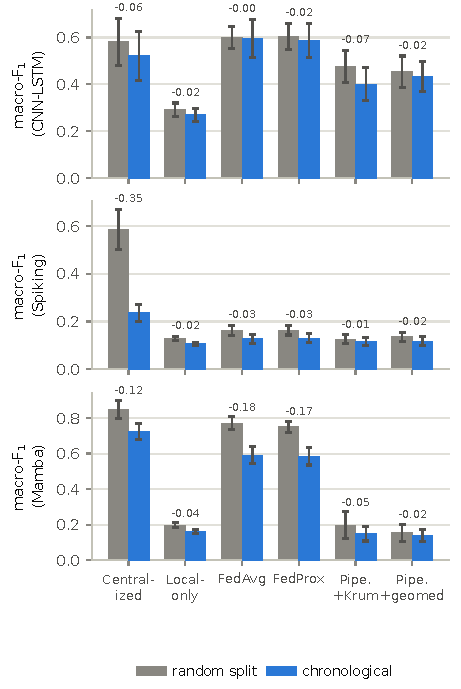
\includegraphics[width=\linewidth]{figures/fig_split_frame}
\caption{Reference-frame \macroF{} (mean $\pm$ sd) per arm and model, chronological split (T1a\_temporal) beside random split (T1a), 15 seeds; numbers give the unpaired change. Cells: Table~\ref{tab:temporal_frame}.}
\label{fig:temporal_frame}
\end{figure}

\paragraph{The margin was leakage: the two dense models tie}
The ranking survives as a tie at the top, not a lead. Under FedAvg the
CNN-LSTM and the state-space model land on each other -- \macroF{}
$0.596$ against $0.590$, a paired difference an exact two-sided Wilcoxon
cannot separate ($p=0.56$) -- and the spiking model sits at $0.128$;
FedProx repeats the shape ($0.587/0.585/0.130$). Most arms lose
$5$--$25\%$ of their random-split score and the floor moves with
everything else; the spiking ceiling loses more (below). The exception
is the federated CNN-LSTM, statistically indifferent to the split
(FedAvg $-0.6\%$, $p=0.89$; FedProx $-2.7\%$): the random
protocol was crediting leakage accuracy to the state-space and spiking
arms and to both bounds, not to the reference. What changes is the claim
-- the state-space model's earlier lead was a margin on leaky cells.

\paragraph{The spiking ceiling was mostly leakage}
The largest single change is not in a federated row: the centralized
spiking ceiling falls $0.586 \rightarrow 0.236$ ($-60\%$) against
$-10\%$/$-15\%$ for the dense ceilings, on matched recipes. The model is
on the floor in \emph{both} regimes ($0.236$ centralized, $0.128$
federated, $0.121$ trivial predictor) -- not a structural limit of
\emph{federated} surrogate-gradient training but the blunter finding
that this architecture does not learn this task at this budget. The
ceiling bounds only two of three arms, too: pooling the CNN-LSTM does
not beat its federated arm ($0.522$ vs.\ $0.596$ chronological, n.s.),
the per-client effective-number reweighting \cite{cui2019} being
miscalibrated on the pooled corpus.

\paragraph{A shallow probe, and the channel it audits}
A deep model is only justified if a cheap one cannot do the job. A
gradient-boosted tree at library defaults reaches \macroF{} $0.692$
pooled and $0.533$ under the chronological cut -- at or above the
CNN-LSTM's \emph{centralized} ceiling under either protocol, so the
reference is justified by timing (Section~\ref{sec:res-latency}), not
centralized accuracy; only its \emph{federated} arm ($0.596$) edges the
pooled probe ($0.692$ leans on default early stopping -- disabled,
$0.275$; detail in Section~\ref{sec:sup-probe}). The same probe audits
the sharpest benchmark shortcut: dropping the synthetic
$f_{\mathrm{dev}}$ channel costs $-0.011$/$-0.027$ \macroF{}
(random/temporal, intervals spanning zero) while the channel alone
reaches $0.295$/$0.234$ -- real but far-from-sufficient signal
(Table~\ref{tab:fdev}). Convergence is in Figure~\ref{fig:rounds}: only
the CNN-LSTM averaging arms reach their ceiling, on every seed.

\subsection{The random split as a leakage-inflated diagnostic}
\label{sec:res-temporal}

What the random split was crediting is visible cell by cell in
Figure~\ref{fig:temporal_attack}: cells carrying real accuracy give up as
much as $0.19$; the pipeline cells barely move, because the random split
only credits accuracy to arms that had accuracy to inflate. The two
results the defense analysis rests on both reproduce under the
controlled protocol: geomed-alone still recovers the loud attacks
(Gaussian noise on the CNN-LSTM: $0.059 \rightarrow 0.541$), and the
full pipeline is still catastrophic against the defense-aware attacker
(pipeline+Krum holds Mamba at $0.051$ where no defense holds $0.553$).
One confound comes with the cut: the test slice moves to a year-end
segment, so every $\Delta$ mixes leakage removal with seasonal shift --
the \emph{differential} pattern argues the leakage term dominates. Both
protocols therefore stay: the random-split battery
(Tables~\ref{tab:frame} and~\ref{tab:attackdefense}) carries the sweeps
and the pre-registered verdicts, and the temporal columns are the ones
to quote for absolute accuracy.

\begin{figure}[tbp]
\centering
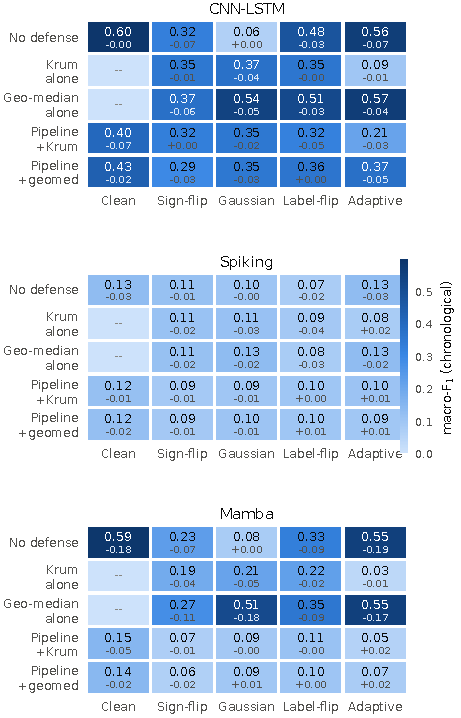
\includegraphics[width=\linewidth]{figures/fig_attack_heatmap}
\caption{Attack $\times$ defense \macroF{}, chronological split (T1b\_temporal, $f_{\mathrm{att}}=3/10$, 15 seeds), one panel per model; second line: change against the random split. Cells: Table~\ref{tab:temporal_attack}.}
\label{fig:temporal_attack}
\end{figure}

\subsection{H1: accuracy parity and the energy ratio}
\label{sec:res-energy}

\begin{figure}[tbp]
\centering
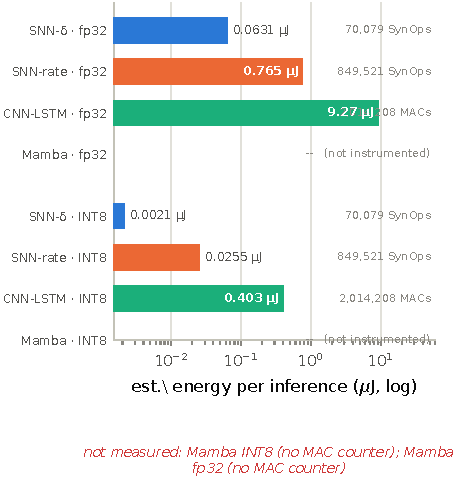
\includegraphics[width=\linewidth]{figures/fig_energy_bars}
\caption{Estimated energy per inference (log scale) per model and coding at $T{=}8$, 45\,nm constants \cite{horowitz2014}. Arithmetic-only SynOps estimate, not a hardware measurement. Cells: Table~\ref{tab:energy}.}
\label{fig:energy}
\end{figure}

The pre-registered parity claim fails decisively: McNemar's exact test
rejects equality ($p<0.001$) and the paired $\Delta$\macroF{} lies far
outside the $\pm0.02$ equivalence margin (BCa 95\% $[-0.465,-0.417]$).
What survives is the energy accounting (Figure~\ref{fig:energy}): under
delta coding the spiking model performs $70\,079$ synaptic operations
per inference against $2\,014\,208$ multiply--accumulates -- an
estimated $0.063$ against $9.27$ microjoules, a ratio $\rho \approx
6.8\times10^{-3}$ with the one-sided BCa interval wholly below one: H1b
is supported, H1a is not, and H1 fails as a conjunction. Rate coding
costs an order of magnitude more for less accuracy
(Section~\ref{sec:res-ablations}); Mamba reads $21.1$\,\uJ{},
$2.3\times$ the reference. These are arithmetic-only estimates, not
hardware measurements. The spiking model delivers its energy reduction
only by conceding almost all of its federated accuracy --
Figure~\ref{fig:energyacc} places every costed arm on the
accuracy--energy plane.

\subsection{Latency against the fast-message envelope}
\label{sec:res-latency}

Inference is one term of the end-to-end chain, so a measured p99 is a
\emph{compute share} of a co-resident 4\,ms fast-message envelope, not a
compliance verdict on it (Figure~\ref{fig:latencyenv}). At fp32 only the
CNN-LSTM leaves any of
the envelope, and only on GPU: $3.28$\,ms p99, $82\%$ of it, against
$212\%$ on CPU; the spiking model ($402$--$423\%$) and Mamba
($548$--$615\%$) exceed the whole envelope alone, and no model benefits
from dynamic INT8 quantization -- torch's kernels reject the recurrent
and state-space packed parameters, so every measured latency is fp32
(distributions in Supplementary Figure~\ref{fig:latency}). The three
architectures resolve into a clean trade-off: Mamba ties for the
accuracy lead but is slowest, the spiking model is cheapest but neither
accurate nor fast, and the reference is the only one whose compute would
fit beside a protection-adjacent function -- on one fixed reference
machine, which orders the models but certifies no substation device.

\begin{figure}[tbp]
\centering
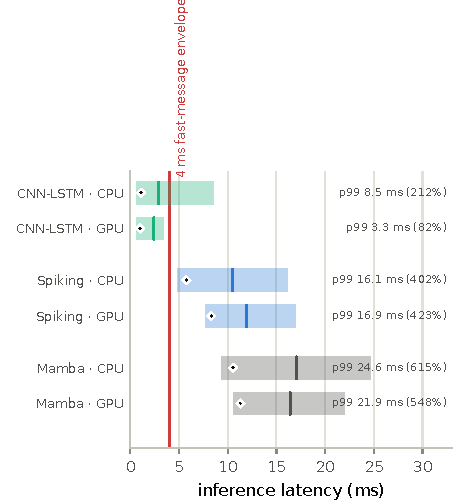
\includegraphics[width=\linewidth]{figures/fig_latency_env}
\caption{Measured inference latency (fp32, batch 1, $n=1000$) per model and device against the 4\,ms fast-message envelope; bar p50--p99, tick p95, diamond mean. A compute share, not compliance. Cells: Table~\ref{tab:latency}.}
\label{fig:latencyenv}
\end{figure}

\subsection{H2: the pipeline under attack}
\label{sec:res-attack}

The grid does not reward the pipeline; this is the paper's central
negative result (Table~\ref{tab:attackdefense}, decomposed rung by rung
in Table~\ref{tab:decomp}). Under the defense-aware attacker,
geometric-median aggregation \emph{alone} preserves accuracy almost
perfectly (CNN-LSTM $-0.020$ from no defense; Mamba $-0.013$) while
rejecting nobody, whereas the same aggregator behind the gate and PBFT
drops to $0.420$/$0.051$ and rejects $66$--$97\%$ of honest updates.
Krum alone is worse than useless -- the single-update selector is
exactly what the cosine-aligned attacker games ($0.043$--$0.100$) -- and
the pipeline compounds the damage: Krum's guarantee needs
$n \ge 2f+3 = 9$ admitted updates at $f=3$, and a gate rejecting most of
the honest population routinely hands it fewer. Under the loud attacks a
robust aggregator recovers most of the loss, the gate never adds
accuracy over the bare aggregator, and Mamba under the adaptive attack
with \emph{no} defense holds $0.739$: it is robust by itself, and the
pipeline takes that away.

The Friedman test agrees under both blockings (Figure~\ref{fig:cd}): at
the pre-registered blocking exactly two pairs separate --
geometric-median-alone above each pipeline arm -- and no-defense against
pipeline+Krum does \emph{not}. Two of the $24$ per-cell tests support
the pipeline after Holm correction (both aggregators against Gaussian
noise on the CNN-LSTM, $\delta=+1.00$) -- loud attacks on the weaker
model, not the defense-aware attacker the pipeline was built for
(Table~\ref{tab:stats}). H2 is recorded as not supported
(Table~\ref{tab:hypotheses}), with the qualification that the agreement
layer contributes the audit record and the measured overhead, not
accuracy; the attack-fraction sweep (T2b) moves the same way.

\subsection{Opening the gate: the admission-threshold sweep}
\label{sec:res-tau}

The pre-registered $\tau=0.5$ is one point on a curve, and sweeping it
changes the diagnosis (Table~\ref{tab:tau_sweep}). As $\tau$ opens to
$1.0$ the gate stops rejecting honest clients (FRR $0.68$--$0.97
\rightarrow \le 0.016$) while the defense-aware attacker is admitted
essentially always ($\ge 0.92$ at $\tau \ge 0.8$) -- the worst of both
worlds on the registered decision rule. What it produces is not: behind
the geometric median accuracy \emph{recovers} as the gate opens
($0.184 \rightarrow 0.487$ pooled; Mamba $0.051 \rightarrow 0.718$,
within $0.01$ of geo-median-alone), while behind Krum it collapses
further ($0.120 \rightarrow 0.069$). This revises H2 rather than
reversing it: at $\tau=0.5$ the gate was \emph{throttling its own
aggregator} -- the negative result is about calibration, not mechanism,
and no setting of $\tau$ makes the pipeline \emph{add} accuracy over the
bare aggregator.

\subsection{H3: the defense-aware attacker's evasion--damage asymmetry}
\label{sec:res-adaptive}

The mechanism behaves exactly as designed, and at fifteen seeds it gets
its statistical answer (Table~\ref{tab:adaptive}). Against either
aggregator the defense-aware attacker holds its realized score to
$0.40$--$0.55$, straddling $\tau=0.5$, where the loud sign-flip scores
$0.98$--$1.05$ and is rejected outright: admission rises from $0.000$ to
$0.53$--$0.59$ and to $0.87$ against Mamba, at
$p_{\mathrm{Holm}} = 1.8\times10^{-4}$ in all six cells -- the evasion is
real and H3a is supported. The same gate still rejects $66$--$98\%$ of
\emph{honest} updates: it does not separate friend from foe, it rejects
both. The damage leg splits by aggregator: behind Krum the admitted
attack costs \emph{more} than the rejected sign-flip on two of three
models ($0.242$ vs.\ $0.153$; $0.167$ vs.\ $0.122$, both significant);
behind the geometric median it runs backwards ($0.034$ vs.\ $0.134$),
because a robust average is not moved by an update it was content to
admit. H3b stays not supported on its $2/6$ cell count -- a property of
the averaging aggregator, not of the test's resolution.

\subsection{The attacker's magnitude lever}
\label{sec:res-magnitude}

\begin{figure}[tbp]
\centering
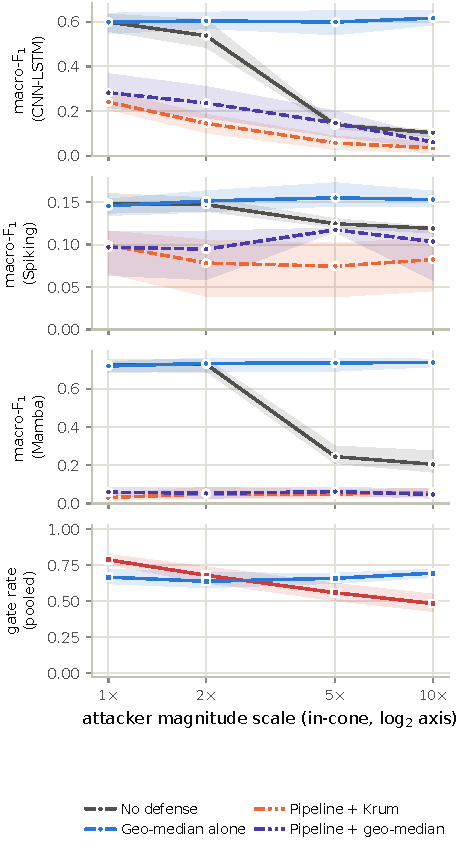
\includegraphics[width=\linewidth]{figures/fig_magnitude}
\caption{\macroF{} (BCa bands) and pooled gate rates as the in-cone attacker scales its update by $s\in\{1,2,5,10\}$ (T4mag, random split, $f_{\mathrm{att}}=3/10$, 9 seeds); $s{=}1$ is the default. Cells: Table~\ref{tab:magnitude}.}
\label{fig:magnitude}
\end{figure}

Cosine scoring is scale-free, so an in-cone attacker can multiply its
update without moving its fidelity score; the pre-registered battery
left that factor at $1$ throughout, and block T4mag sweeps it
(Figure~\ref{fig:magnitude}). Three things happen, and they point the
same way. \emph{Plain averaging breaks}: the undefended CNN-LSTM falls
$0.598 \rightarrow 0.103$ and Mamba $0.727 \rightarrow 0.205$ --
significant at $5\times$--$10\times$ on the dense models, descriptively
the damage leg H3b failed to find at unit magnitude. \emph{The geometric
median is invariant to the lever}: its cells move by at most $+0.019$, a
breakdown-point argument appearing as a measurement. \emph{The gate
loosens under the lever}: the attacker's score barely moves
($0.466 \rightarrow 0.417$) while honest false-rejection falls
$0.799 \rightarrow 0.476$ -- the honest population's own mean score
slides through the fixed threshold ($0.608 \rightarrow 0.470$),
collapsing the discriminative gap ($0.142 \rightarrow 0.052$). The gate
loosens not because the attacker climbs toward the threshold but because
the honest clients slide down through it; neither gated arm profits.

\subsection{H4: the privacy-versus-admission operating curve}
\label{sec:res-ldp}

\begin{figure}[tbp]
\centering
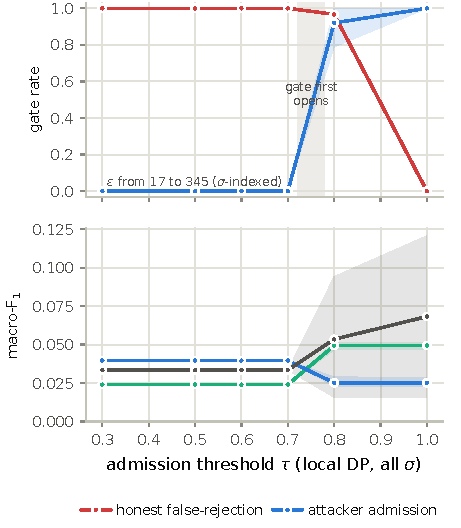
\includegraphics[width=\linewidth]{figures/fig_ldp_tau}
\caption{Gate rates (top) and \macroF{} (bottom) against $\tau$ on pipeline+Krum under the defense-aware attacker, pooled over four $\sigma$ (band: cross-$\sigma$ range; T2c and T3$\tau$, random split, 9 seeds). Cells: Table~\ref{tab:ldp_tau_extended}.}
\label{fig:ldp_tau}
\end{figure}

The operating curve is degenerate, and the extended sweep shows why
(Figure~\ref{fig:ldp_tau}). Across all twelve registered
$(\sigma,\tau)$ points the honest false-rejection rate is pinned at
$1.000$ and the attacker admission reads $0.000$ only because
\emph{nothing} is admitted -- the gate rejects all ten clients in all
thirty rounds, the model never leaves initialization, and the reported
\macroF{} is an untrained network's, below even the $0.121$ majority
floor; the ordered-trend test is correspondingly flat
(Jonckheere--Terpstra $p=0.500$), so H4 is not supported. The gate first
opens between $\tau=0.7$ and $0.8$; past it the attacker is admitted
$0.788$--$1.000$ and \macroF{} stays on the floor: no corner that was
run buys the accuracy back (two caveats: the extension is pipeline+Krum
only, and six runs diverged on non-finite scores -- excluded, ``div.'').
The argument is dimensional, not a tuning failure: on $\sim
10^{5}$-parameter updates, isotropic noise calibrated for local DP must
overwhelm the update direction entirely -- the scored cosine becomes
noise -- and even the weakest setting carries a near-vacuous budget
($\varepsilon$ from $16.9$ to $345$). Update-level local DP and cosine
admission are, on this architecture, mutually exclusive: a
near-impossibility we quantify rather than a curve we tune.

\subsection{H5: heterogeneity}
\label{sec:res-alpha}

Heterogeneity degrades the two weaker models and leaves the state-space
model alone -- not the pre-registered prediction
(Table~\ref{tab:alpha}). From the near-uniform control to
$\alpha = 0.1$, FedAvg CNN-LSTM \macroF{} falls $0.683 \rightarrow
0.499$ and FedAvg spiking $0.190 \rightarrow 0.118$, while FedAvg Mamba
does not move outside seed noise ($0.770 \rightarrow 0.798$, in the
wrong direction). Four of six ordered-trend tests survive Holm
correction -- both weaker models on both arms -- while both Mamba trends
stay flat at $n=42$ runs per trend, so H5a fails its decision rule on
architecture, not power. H5b fails too: exactly one of three cells
clears the floor (spiking, $\delta=+0.88$), the CNN-LSTM cell inverts
($\delta=-0.51$) and Mamba's is flat. The conjunction fails on both legs
for two different reasons; the state-space model is simply insensitive
to label skew over the swept range -- a finding, not a failure.

\subsection{Consensus overhead}
\label{sec:res-consensus}

At the default committee a committing round costs exactly $180$ messages
and $167.8$\,ms of simulated wide-area latency against a training round
orders of magnitude longer, so agreement is not the bottleneck
(Table~\ref{tab:consensus}). The sweep's accuracy reading is no
robustness story: pipeline+Krum is already collapsed at every committee
size, and the moves between $M \in \{4,7,10\}$ are seed variance of a
collapsed arm -- overhead without accuracy return at this operating
point. And the auditability claim is bounded exactly: pipeline arms
append every round to a SHA-256 chain, but no \texttt{RunResult}
carries an end-to-end verification, so auditability is a design claim
with property-test coverage, not a measurement; the latency is a lower
bound (Section~\ref{sec:threat}).

\subsection{Per-class behaviour}
\label{sec:res-perclass}

\begin{figure}[tbp]
\centering
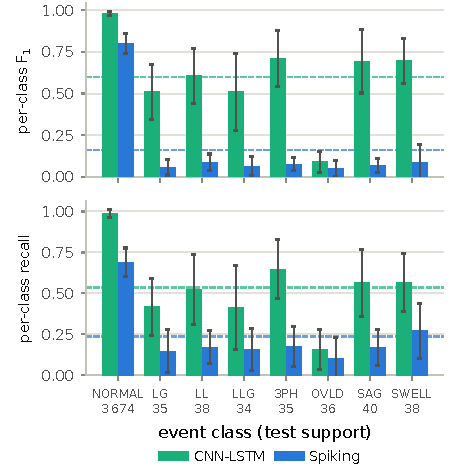
\includegraphics[width=\linewidth]{figures/fig_perclass}
\caption{Per-class F\textsubscript{1} and recall (mean $\pm$ sd; dashed: macro score) with mean test support, clean FedAvg reference (T1a, random split, 15 seeds). Cells: Table~\ref{tab:perclass}.}
\label{fig:perclass}
\end{figure}

The macro average hides a rare-event problem
(Figure~\ref{fig:perclass}). At the clean FedAvg reference the CNN-LSTM
carries \cls{normal} almost perfectly ($F_1 = 0.983$) but degrades on
the fault and power-quality classes whose support is in the tens -- down
to $F_1 = 0.089$ on \cls{overload} -- so its $0.600$ is a rare-class
average. The spiking model fails these outright: on \cls{fault\_lg} its
recall of $0.147$ comes with near-zero precision -- the collapsed model
sprays the rare label rather than never predicting it. These are
statements about class rarity, not intrinsic detectability.

\subsection{Ablations and the real-trace sanity check}
\label{sec:res-ablations}
\label{sec:res-real}

Neither ablation rescues the spiking collapse or improves on FedAvg
(Tables~\ref{tab:coding} and~\ref{tab:fedprox}). Under delta coding,
shortening the unroll helps -- $T=4$ gives the best clean \macroF{} at
$0.204$ against $T=8$'s $0.161$ -- so longer integration buys more
SynOps for \emph{less} accuracy, and rate coding pins at the trivial
floor; the most favourable spiking configuration sits at about a quarter
of Mamba's federated \macroF{}. FedProx is inert (largest paired gain
$+0.006$; Mamba at $\mu=0.1$ loses $0.150$). On the MSU/ORNL real
traces -- a sanity check read narrowly: near-IID, effectively binary,
random split, $n=3$ -- every arm runs to completion and the ordering
\emph{inverts} (spiking $0.996$, Mamba $1.000$, CNN-LSTM $0.703$;
pipeline $0.927$--$0.990$ on the spiking and Mamba models,
$0.486$--$0.726$ on the CNN-LSTM): the pipeline is operable on real
IEC~61850-adjacent traces, but the set does not validate the synthetic
benchmark.

\subsection{Statistical battery and hypothesis verdicts}
\label{sec:res-stats}

Table~\ref{tab:stats} collects the complete battery and
Table~\ref{tab:hypotheses} the verdicts, and the scoreboard is
unflattering but fully decidable: exactly two hypotheses are supported
-- H1b (the spiking energy ratio below one) and H3a (the defense-aware
evasion) -- while H1a, H2, H3b, H4, H5a and H5b are not, and the
conjunctions fail with them; none is a power artefact any more. What the
tables do support is an open, honestly scored benchmark carrying four
durable findings: a three-corner model trade-off whose accuracy corner
is \emph{shared} between the two dense models; a negative result on
elaborate Byzantine admission -- robust averaging alone suffices and the
gate buys auditability, not accuracy; an unpredicted heterogeneity
result -- the co-leading architecture is indifferent to label skew; and
the one attack that breaks plain averaging -- in-cone magnitude --
against which the geometric median is invariant and the gate loosens.

\section{Discussion}
\label{sec:discussion}

The interpretive frames in this section were fixed with the
pre-registration, before any result existed, and are not adjusted to what
the battery returned: where the result contradicts the registered
expectation -- and in three places it does -- the frame is kept and the
expectation is the thing that goes.

\subsection{A three-way trade-off, not a single winner}

The central picture is a trade-off, and the honest reading names the
corner each architecture occupies -- and on the headline chronological
split the accuracy corner is \emph{shared}, not held: the
convolutional--recurrent reference and the selective state-space model
tie at \macroF{} $0.596$ and $0.590$ ($p=0.56$). The state-space model
adds the highest centralized ceiling ($0.724$) at the largest compute
($21.1$\,\uJ{} arithmetic-only, p99 $>5\times$ the co-resident envelope).
The reference model is the \emph{timing} choice: statistically
indistinguishable accuracy, the only model whose p99 leaves any of that
envelope ($82\%$, GPU only). The spiking model is the \emph{energy}
choice: about $147\times$ cheaper by SynOps accounting, but collapsed to
$0.128$ federated and $0.236$ centralized -- it does not learn this task
at this budget. A deployment picks a corner; the benchmark's
contribution is to make the corners measurable on a common substrate.
Even that reading is complicated by the probe: the reference is not
justified by \emph{centralized} accuracy -- only its federated arm edges
the pooled probe.

\subsection{Mechanisms: what happened, why, and what follows}
\label{sec:mechanisms}

Four findings earn their keep only if their mechanism is stated.

\paragraph{The random split inflates accuracy}
\emph{What:} every arm scored higher under the random permutation
(the federated CNN-LSTM only within seed noise, $-0.6\%$) -- the spiking
centralized ceiling by $60\%$ -- and the
leakage-controlled split took it back. \emph{Why:} neighbouring windows
share $75\%$ of their samples, so a high-capacity classifier on
near-duplicate windows is doing lookup, not generalization.
\emph{Implication:} quote the chronological columns; the random split is
kept as the diagnostic showing what an uncontrolled split credits to
leakage -- up to $0.19$ \macroF{} on the cells that had accuracy to
inflate.

\paragraph{Physical heterogeneity looks Byzantine to a direction gate}
\emph{What:} at $\tau=0.5$ the gate rejected $66$--$98\%$ of
\emph{honest} updates while admitting the defense-aware attacker half
the time. \emph{Why:} the score is cosine distance to the round's
median, and this federation is non-IID by construction -- different
feeders, load mixes and event populations push honest updates in
legitimately different directions, and local-DP noise makes the same
confusion literal. \emph{Implication:} a direction-only statistic cannot
separate the federation's own heterogeneity from malice; if a gate is
deployed at all, calibration matters more than the statistic.

\paragraph{The admission gate degrades the robust aggregator by
starving it}
\emph{What:} geometric-median aggregation alone holds its accuracy under
the defense-aware attacker ($0.609$/$0.726$) while the same aggregator
behind the gate drops to $0.420$/$0.051$. \emph{Why:} a robust average
needs honest mass, a selector needs honest neighbours, and at
$\tau=0.5$ the gate discards most of the honest population -- Krum's
$n \ge 2f+3$ condition is routinely unmet; opened to $\tau=1.0$ the
same gate costs almost nothing. \emph{Implication:} a gate in front of a
robust aggregator must be calibrated to admit; a gate that rejects most
of the honest population is a denial-of-service on its own federation.

\paragraph{Accuracy, privacy, energy and latency pull in different
directions}
\emph{What:} no arm takes every axis -- the accuracy lead is shared
between the only model that fits the timing envelope and the slowest
model, while the cheapest per inference is the least accurate.
\emph{Why:} the desiderata bind different resources -- capacity, sparse
arithmetic, a compiled kernel, isotropic noise the direction gate cannot
tell from an attack, and a jointly witnessed decision whose
$180$-message round buys a record, not accuracy. \emph{Implication:}
deployment chooses a corner, which is also why geometric-median-alone is
the defensible default for the defense axis.

\subsection{Energy against accuracy: what the ratio does not say}

Three things must be read together. \emph{First}, parity is a premise,
not a bonus, and it failed -- the paired $\Delta$\macroF{} interval
$[-0.465,-0.417]$ sits far outside the $\pm0.02$ margin, so the energy
comparison runs between models at different operating points; the
literature had made parity look plausible \cite{mahapatra2021}, which is
exactly why the negative result is worth reporting. \emph{Second}, the
ratio is arithmetic-only at 45\,nm constants \cite{horowitz2014},
excluding memory traffic -- often the dominant term. \emph{Third},
coding moves both axes at once: temporal-contrast emits events only
where the signal changes -- a strong prior on quasi-static telemetry --
and is twelve times cheaper than rate coding \emph{and} the only coding
above the trivial floor, while thresholds below $0.1$ fire on the
instrument noise.

\subsection{The defense asymmetry}

The evasion half of the asymmetry is now decided rather than descriptive
-- admission rises from $0.000$ to $0.53$--$0.87$ at
$p_{\mathrm{Holm}} = 1.8\times10^{-4}$ in every cell -- and the damage
half splits on the aggregator: behind Krum the admitted attack costs
measurably more than the rejected one on two of three models, while
behind the geometric median it runs backwards, because a robust average
is not moved by an update it was content to admit. The conclusion is
narrower than the hypothesis and more useful: evading a cosine gate is
easy and, against a robust average, close to pointless \emph{at honest
magnitude}.

The magnitude lever removes that qualification. What makes a single
cosine threshold portable -- scale-freeness -- is exactly what makes it
blind to norm: admitted magnitude translates directly into displacement,
and plain averaging does not survive the lever ($0.598 \rightarrow
0.103$) while the geometric median barely registers it. The design
recommendation therefore collapses to something simpler than the one we
set out with: \emph{deploy the geometric median on its own} -- the only
arm robust to the attack the gate cannot see -- and if a cosine gate is
kept for the auditable record, it needs a norm bound, which is a
clipping rule, not an admission rule. A second, untested direction
follows from the attacker's aiming error: an admission statistic not
estimable from public information alone would widen that error and
narrow the usable cone without changing the interface.

\subsection{What the agreement layer buys, and what privacy costs}

Byzantine agreement is not an accuracy mechanism here; what it remains
is a \emph{governance} mechanism -- it makes the admission decision
jointly witnessed rather than a server's private choice, and appends a
hash-chained record, which in a federation of competing utilities is
what a regulator or contractual counterparty asks for. The guarantee is
bounded twice over: the chain is tamper-evident but does not stop a
writer who re-hashes every successor, and this battery builds it in
memory and discards it, so auditability is a design claim, not a
measurement. The cost side rides in the same breath: the overhead
figures are a \emph{lower bound} (always-honest primary, no view change,
no authentication).

On privacy the selection procedure has no solution on this architecture,
because the curve is a point: at every $\tau \le 0.7$ the gate rejects
all ten clients in all thirty rounds; at $\tau \ge 0.8$ it admits the
attacker essentially always and \macroF{} stays at or below the trivial
floor, at near-vacuous $\varepsilon$ throughout -- consistent with the
theory \cite{guerraoui2021podc} and an argument for the designs that
route around the tension \cite{gu2024dpbrem}: server-side or distributed
noise, or admission on a quantity that survives isotropic perturbation.

\subsection{Implications for a utility consortium}

Read together, the frames suggest a deployment shape rather than a
product. Federation is worth it: every federated arm beats its
local-only floor under both protocols. Robust aggregation should be
\emph{selected} rather than composed -- geometric-median-alone was the
best-ranked defense arm and every layer on top cost accuracy; if an
admission gate is deployed anyway, for auditability, it must be
calibrated to admit. Agreement should be justified on governance, with
its chain actually persisted and verified, which this battery did not
do. Update-level privacy should not be composed with cosine admission on
architectures of this size. And one recommendation reverses on the
evidence: heterogeneity was expected to be the binding constraint, but
the state-space model does not move across the swept skew -- a
consortium expecting severe label skew has an architectural answer
before it has a federated-algorithm one. Whether that indifference
survives beyond the swept range and beyond ten clients, we do not know;
and the classifier should be chosen for the envelope of the hardware
installed in the bay -- an argument for evaluating event-driven models
on event-driven hardware.

\section{Limitations and conclusion}
\label{sec:limitations}

We list limitations at the granularity at which they could change a
conclusion; each is a thing a reader should know before citing a number
from this paper.

\subsection{Limitations}
\label{sec:limitations-list}

\paragraph{Energy is an estimate, not a measurement}
SynOps accounting prices counted synaptic events and analytic
multiply--accumulate counts at published 45\,nm constants
\cite{horowitz2014} -- arithmetic only, excluding memory access, data
movement and peripherals, which on many accelerators dominate; the dense
reference is analytic too, and no power was measured on any device.

\paragraph{The consensus overhead is a lower bound, and the ledger is
not persisted}
The primary is always honest, so no view change occurs; message
authentication, batching, checkpointing and garbage collection are not
priced; the wide-area latency distribution is fitted-synthetic
\cite{aikat2003}; and validators are simulated processes
in one host. There is one in-memory chain, not one replica per
validator, and no \texttt{RunResult} field persists it -- chain
integrity is covered by property tests, not by these runs.

\paragraph{Simulated data, not field data}
Every synthetic window comes from a physics simulator; the
fitted-synthetic rows are named in the realism audit
(Tables~\ref{tab:realism}--\ref{tab:realism2b}). The 60\,s quasi-static
cadence is the largest single simplification -- sub-minute clearing
sequences are unobservable, so episodes represent what one-minute RMS
telemetry captures, not point-on-wave behaviour. No protection equipment
is modelled: faults persist for their full drawn duration, so fault
windows are more observable than in the field and fault-class accuracies
are optimistic. Absolute \macroF{} values outside the
chronological-split tables are likewise optimistic ceilings -- the
sweeps, ablations and local-DP grid were not re-run under the controlled
protocol. The $f_{\mathrm{dev}}$ channel is synthetic and event-coupled
-- a possible label shortcut, bounded by the probe ablation of
Section~\ref{sec:res-frame} on a shallow model only. Fault location is
bus-granular, photovoltaic modelling simplified, windows do not cross
day boundaries, the class prior is a modelling choice, and one solver
produced every window.

\paragraph{Scope of the battery}
Seeds are fifteen at Tier~1 and the temporal controls, nine elsewhere,
and the extension mixes two execution environments -- bounded by a
homogeneous-subset analysis and fixed by dated amendment. The client
count is fixed at ten; the heterogeneity control is near-uniform, not
uniform; hyperparameters were tuned once on clean FedAvg and frozen, so
the spiking collapse is a collapse \emph{at this optimization budget} --
a per-architecture search remains a live alternative explanation; no
model was quantized; the temporal and magnitude batteries are
post-registration controls; and root-dataset trust bootstrapping
\cite{cao2021fltrust} is excluded by assumption, cited not re-run.

\paragraph{Threat model}
Label-flip is dynamic per-batch noise, a weaker, higher-variance
adversary than static poisoning. The adaptive attacker is defense-aware
but not omniscient and never observes $\tau$, so the H3b null does not
separate an under-powered attacker from a working defense; the cone
angle $\varsigma$ is never swept, so measured evasion is a lower bound;
it wastes its first round by construction; adversary placement is
structured and static; a single non-finite submission can deny the
defense for a round -- an open vulnerability we name rather than
measure; Krum's $n \ge 2f+3$ guarantee is void behind a tight gate; and
the attacker blinds itself on a fail-closed round.

\paragraph{Reproducibility and per-class rarity}
Bit-reproducibility is claimed on CPU only; per-run git provenance is
mostly absent, so regeneration rests on manifests, configuration hashes
($66.7\%$ re-verifying canonically on the original battery) and seeded
determinism (Section~\ref{sec:sup-provenance}). The rarest fault class
has single-digit support in some splits, so its recall is unstable and
reported rather than smoothed -- detecting it reliably needs a different
sampling design.

\subsection{Conclusion}
\label{sec:conclusion}

\sysname{} treats the four constraints of federated substation event
classification -- data that cannot be pooled, physical heterogeneity, an
energy- and latency-bounded edge, and a federation with no trusted party
-- as one design problem, and stress-tests it end to end rather than
claiming it robust. The programme was pre-registered and reported
against its own decision rules, and several rules returned negative --
which is the point of pre-registering them. On the leakage-controlled
chronological split the two dense architectures tie at the top
(\macroF{} $0.596$/$0.590$); the spiking model, two orders of magnitude
cheaper in estimated energy, is on the floor federated \emph{and}
centralized -- it does not learn this task at this budget. The admission
pipeline, ablated against the robust aggregator standing alone, buys an
auditable, jointly witnessed decision rather than accuracy; local DP and
cosine admission are incompatible at every usable privacy level;
heterogeneity leaves the state-space model unmoved across the whole
swept skew; the consensus layer's cost is a lower bound next to the
accuracy it does not buy; and the auditability it does buy is a design
property, not a measurement. Three directions follow: move the energy
claim from analytic accounting to event-driven hardware; add a norm
bound -- or a statistic not estimable from public information -- to any
deployed cosine gate, since magnitude is the lever that breaks plain
averaging while the geometric median absorbs it untouched; and release
the generator's federations at SMART-DS scale \cite{smartds}, so
federated grid learning can be compared on a common, physically grounded
substrate.

\section*{Data availability}
\addcontentsline{toc}{section}{Data availability}

All data behind the paper's primary results are \emph{generated} by the
quasi-static OpenDSS simulation with synthetic event and measurement
overlays described in Section~\ref{sec:testbed}, released as part of the
software artifact together with the unmodified public test-feeder models
it consumes \cite{kersting2001} (BSD-3-Clause licence). One third-party
dataset is used, and only for the real-trace sanity check of
Section~\ref{sec:res-real}: the public MSU/ORNL power-system attack and
disturbance dataset, used unmodified under its published terms; it
supports no model or defense comparison in this paper. The federations
behind every reported synthetic result are reproducible from source with
a fixed seed:

\begin{quote}\scriptsize\ttfamily\raggedright
python -m experiments.stage\_data --out data\_battery\\
python -m experiments.run\_all --dry-run\\
python -m experiments.gen\_temporal\_battery\\
python -m experiments.gen\_magnitude\_sweep\\
python -m experiments.manifest\_tau\\
python -m experiments.gen\_gap\_x3\\
python -m experiments.run\_all --data-dir data\_battery\\
\mbox{}\quad --out-dir runs --device cuda\\
python -m experiments.report --runs-dir runs\_snn\_fixed runs\\
\mbox{}\quad runs\_x3 runs\_ssm\_x3 runs\_gap\_x3\\
\mbox{}\quad --tables-dir paper/tables --summary runs/summary.json
\end{quote}

The first regenerates the labelled per-substation windows; the second
enumerates every pre-registered run with its configuration hash; the next
four re-emit the post-registration batteries as committed manifests (the
chronological split, the magnitude, threshold and X3 gap sweeps; the
remaining X3 manifests ship committed like the rest), all regenerating
canonically; the last two execute the battery and rebuild the merged
corpus, the tables and the statistical battery, deduplicating first by
\texttt{run\_id} and then on a semantic configuration key. The generator,
the generated federations, all per-run result records, the run manifest
and the figure and table scripts are deposited in the public archive
identified below, so that the tables and figures of
Section~\ref{sec:results} can be rebuilt without re-running the battery.

\section*{Code availability}
\addcontentsline{toc}{section}{Code availability}

The complete framework -- simulation, models, federated engine, attack
suite, consensus pipeline, experiment runner, analysis code and tests --
is open source, together with the generated federations and every per-run
result record, at \url{https://github.com/ufxa/gridspike} (code under
MIT, data and results under CC BY 4.0); an archived release with a
persistent identifier will be cited here on acceptance. The
package keeps its development name (\texttt{fedgrid}) in the repository;
the system is named \sysname{} in this manuscript because that name is
already in use for an unrelated published system.

\section*{Declaration of competing interest}
\addcontentsline{toc}{section}{Declaration of competing interest}

\TODOnum{competing-interest statement: authors to confirm on the title page}
The authors declare that they have no known competing financial interests or
personal relationships that could have appeared to influence the work reported
in this paper. (The definitive statement, with author names, is on the separate
title page.)

\section*{Funding}
\addcontentsline{toc}{section}{Funding}

\TODOnum{funding sources: authors to confirm on the title page}
The definitive funding statement, including grant numbers where applicable, is
on the separate title page. If the work received no specific grant from funding
agencies in the public, commercial or not-for-profit sectors, that is stated
there.

\section*{CRediT authorship contribution statement}
\addcontentsline{toc}{section}{CRediT authorship contribution statement}

Author contributions are recorded using the CRediT taxonomy on the separate,
non-anonymized title page, as required by the double-anonymized review model.

\section*{Declaration of generative AI and AI-assisted technologies in the manuscript preparation process}
\addcontentsline{toc}{section}{Declaration of generative AI and AI-assisted technologies}

During the preparation of this work, the author(s) used
\TODOnum{name of tool / service} in order to
\TODOnum{reason: e.g.\ draft and edit sections of the manuscript}. After using
this tool/service, the author(s) reviewed and edited the content as needed and
take(s) full responsibility for the content of the published article.

\medskip
\noindent\emph{Note.} Use of artificial intelligence \emph{within the research
methodology itself} is disclosed separately in
Section~\ref{sec:ai-methodology}, in accordance with the publisher's policy that
methodological AI use belongs in the Methods rather than in this statement. No
AI system is listed as an author, and no AI-generated image is presented as
primary research data.


\bibliographystyle{elsarticle-num}
\bibliography{refs}

\end{document}
